

\subsection{Đánh giá hiệu năng hệ thống nâng cao}
Sau khi hoàn tất quá trình tổng hợp (Synthesis) trên Vivado, nhóm tiến hành thu thập và phân tích các thông số hiệu năng của phiên bản CPU nâng cao, bao gồm tài nguyên phần cứng, thời gian và năng lượng tiêu thụ.

\subsubsection{Phân tích tài nguyên sử dụng (Utilization Report)}

\begin{figure}[H]
    \centering
    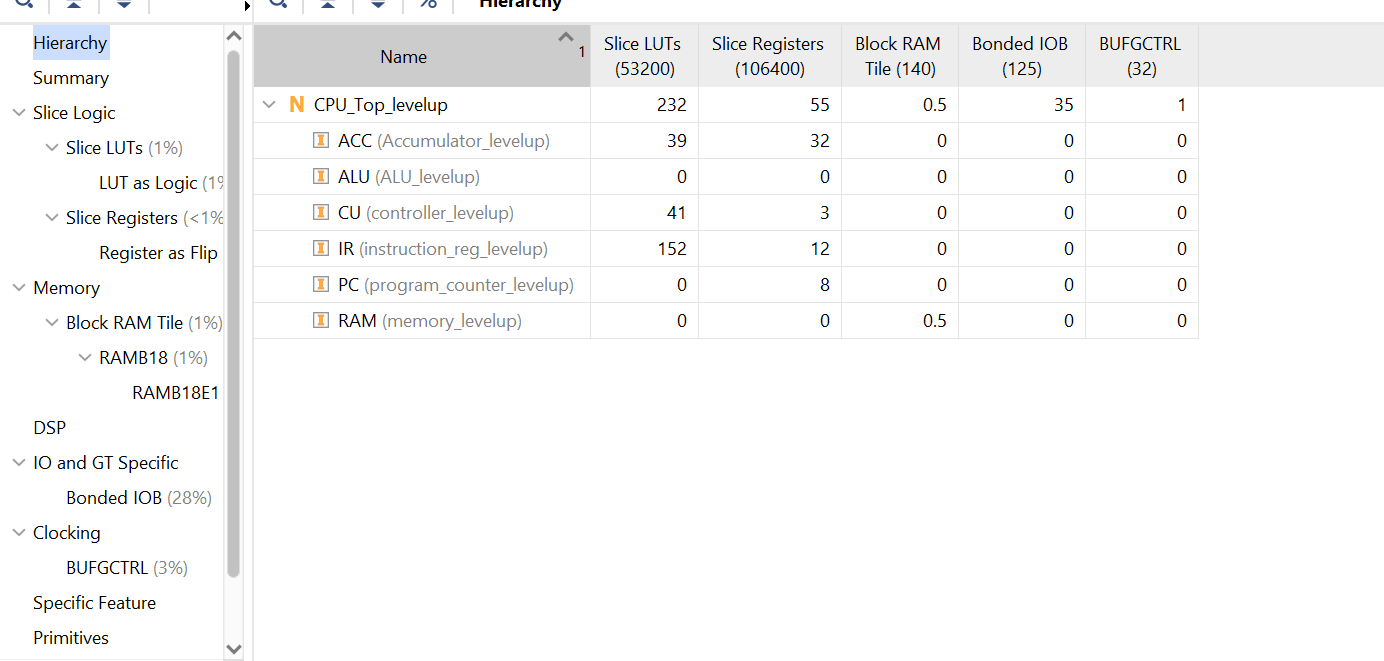
\includegraphics[width=1.0\textwidth]{til1.png} 
    \caption{Báo cáo tài nguyên Utilization chi tiết cho từng module (phiên bản nâng cao)}
    \label{fig:util_report}
\end{figure}

\begin{table}[H]
\centering
\footnotesize % Dùng mức nhỏ hơn small để an toàn tuyệt đối
\setlength{\tabcolsep}{3pt} % Thu hẹp khoảng cách giữa các cột
\begin{tabularx}{\textwidth}{|X|c|c|c|c|c|} % Cột đầu tiên tự co giãn
\hline
\textbf{Module} & \textbf{LUTs} & \textbf{Registers} 
& \textbf{BRAM} & \textbf{IOB} & \textbf{BUFG} \\
\hline
CPU\_Top\_levelup        & 232 & 55  & 0.5 & 35 & 1 \\
ACC (Accumulator)        & 39  & 32  & 0   & 0  & 0 \\
ALU (ALU\_levelup)       & 0   & 0   & 0   & 0  & 0 \\
CU (controller)          & 41  & 3   & 0   & 0  & 0 \\
IR (instruction)         & 152 & 12  & 0   & 0  & 0 \\
PC (prog\_counter)       & 0   & 8   & 0   & 0  & 0 \\
RAM (memory)             & 0   & 0   & 0.5 & 0  & 0 \\
\hline
\end{tabularx}
\caption{Báo cáo tài nguyên phiên bản CPU nâng cao}
\label{tab:util_levelup}
\end{table}

\textbf{Nhận xét:} \\
Hệ thống nâng cao tiêu thụ tổng cộng 232 LUTs và 55 Registers, tăng đáng kể so với phiên bản cơ bản (130 LUTs, 54 Registers). Sự gia tăng này chủ yếu đến từ các nguyên nhân sau:
\begin{itemize}
    \item \textbf{Khối IR:} Tăng mạnh nhất (từ 51 lên 152 LUTs) do phải xử lý opcode 4-bit và địa chỉ 28-bit. Việc mở rộng trường opcode khiến logic giải mã phức tạp hơn.
    \item \textbf{Khối CU:} Tăng nhẹ phản ánh việc bổ sung logic điều chỉnh cho 7 lệnh mới.
    \item \textbf{Khối ALU:} Tiêu thụ 0 LUTs do Vivado tối ưu hóa thành các primitives có sẵn.
    \item \textbf{Khối RAM:} Ánh xạ vào 0.5 Block RAM Tile, giữ nguyên so với phiên bản cơ bản.
\end{itemize}

Bảng dưới đây so sánh tài nguyên giữa hai phiên bản:

\begin{table}[H]
\centering
\begin{tabular}{|l|c|c|c|}
\hline
\textbf{Tiêu chí} & \textbf{Phiên bản cơ bản} & \textbf{Phiên bản nâng cao} & \textbf{Tăng} \\
\hline
Slice LUTs      & 130  & 232  & +78\% \\
Slice Registers & 54   & 55   & +2\%  \\
Block RAM Tile  & 0.5  & 0.5  & 0\%   \\
Bonded IOB      & 3    & 35   & +1067\% \\
\hline
\end{tabular}
\caption{So sánh tài nguyên phiên bản cơ bản và nâng cao}
\label{tab:util_compare}
\end{table}

Sự tăng vọt của \textbf{Bonded IOB} (từ 3 lên 35) phát sinh từ việc bổ sung ngõ ra \texttt{acc\_val[31:0]} (32 chân) để hiển thị kết quả ra LED trên FPGA.

\subsubsection{Phân tích thời gian (Timing Analysis)}

\begin{figure}[H]
    \centering
    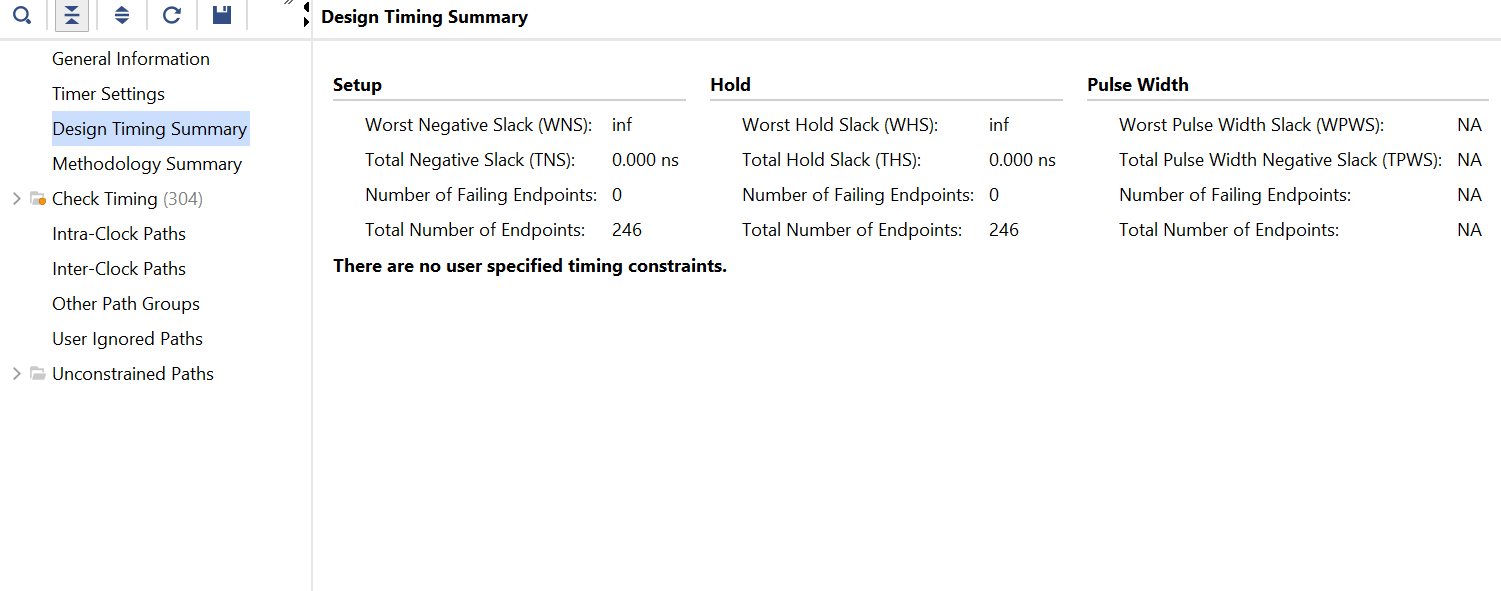
\includegraphics[width=1.0\textwidth]{timing.png} 
    \caption{Báo cáo phân tích thời gian Timing Summary (phiên bản nâng cao)}
    \label{fig:timing_report}
\end{figure}

\textbf{Nhận xét:}
\begin{itemize}
    \item Chỉ số \textbf{TNS (Total Negative Slack)} bằng 0.000 ns, khẳng định thiết kế không vi phạm ràng buộc thời gian hoặc lỗi chạy đua tín hiệu.
    \item Tổng số Endpoints tăng từ 211 lên 246 do bổ sung tập lệnh mới.
    \item Hệ thống hoàn toàn đáp ứng các ứng dụng yêu cầu tần số hoạt động tiêu chuẩn trên chip Artix-7.
\end{itemize}

\subsubsection{Phân tích năng lượng tiêu thụ (Power Analysis)}

\begin{figure}[H]
    \centering
    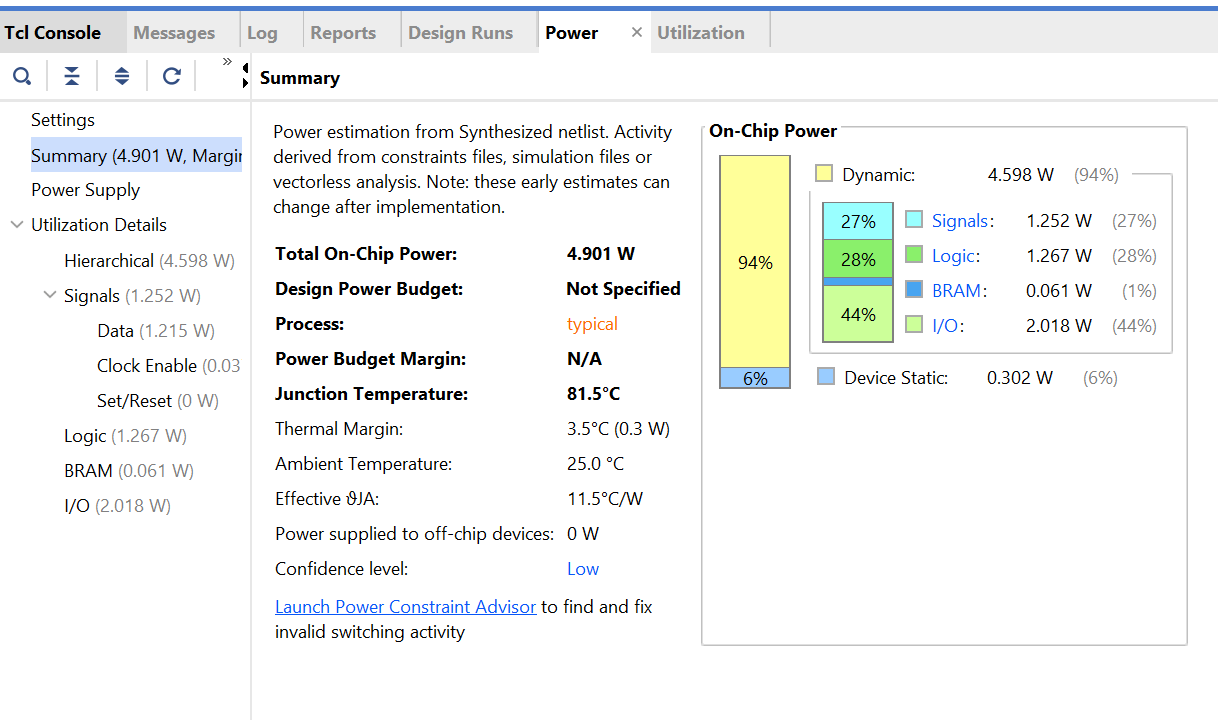
\includegraphics[width=0.9\textwidth]{pow.png} 
    \caption{Báo cáo ước tính năng lượng tiêu thụ (phiên bản nâng cao)}
    \label{fig:power_report}
\end{figure}

\textbf{Nhận xét:}
\begin{itemize}
    \item \textbf{Tổng công suất:} Đạt 4.901 W (tăng so với 1.952 W ở bản cơ bản). Nguyên nhân chính là do I/O chiếm tới 44\% (do 32 chân \texttt{acc\_val}).
    \item \textbf{Nhiệt độ Junction:} Đạt 81.5°C, vẫn nằm trong giới hạn an toàn ($< 85$°C) nhưng cần lưu ý về tản nhiệt khi triển khai thực tế.
\end{itemize}

Bảng dưới đây tổng hợp so sánh hiệu năng giữa hai phiên bản:

\begin{table}[H]
\centering
\small
\begin{tabular}{|l|c|c|}
\hline
\textbf{Thông số} & \textbf{Phiên bản cơ bản} & \textbf{Phiên bản nâng cao} \\
\hline
Tổng công suất       & 1.952 W  & 4.901 W  \\
Công suất động       & 93\%     & 94\%     \\
Công suất I/O        & 0.194 W  & 2.018 W  \\
Nhiệt độ Junction    & 47.5°C   & 81.5°C   \\
Thermal Margin       & 3.1°C    & 3.5°C (0.3 W) \\
TNS                  & 0.000 ns & 0.000 ns \\
Failing Endpoints    & 0        & 0        \\
Tổng Endpoints       & 211      & 246      \\
\hline
\end{tabular}
\caption{So sánh hiệu năng tổng thể giữa hai phiên bản CPU}
\label{tab:perf_compare}
\end{table}

